% kapitel2.tex
\section{Der Aufbau und die Fertigung}
\label{chapter:kap1}
\subsection{Die technischen Komponenten}
In Tabelle 1 sind die verbauten Komponenten des Spiegels aufgelistet und werden in den darauf folgenden Kapiteln näher beschrieben. Das Material wurde von unterschiedlichen Quellen bezogen. Die jeweilige Bezugsquelle ist in der Spalte ,,Link`` verlinkt. Neben der Bezugsquelle ist der Einkaufpreis des Materials gelistet. Die Komponenten sind in zwei Gruppen aufgeteilt. Die Gruppe, bestehend aus der Spiegeleinheit und der Displayeinheit, die für die Herstellung des Spiegels selbst notwendig ist und die Gruppe, bestehend aus der Recheneinheit, welche im Spiegel verbaut ist und dem Spiegel seine Funktionalität ermöglicht.
\begin{table}[H]
	\scriptsize
	\begin{tabular}{r|l|l|r}
		& \textbf{Komponente} & \textbf{Link} & \textbf{Preis €} \\
		\hline
		\multirow{4}{*}{\textbf{Spiegeleinheit}} & IKEA RIBBA Rahmen, schwarz &
		\href{http://www.ikea.com/de/de/catalog/products/00078051/#/20078050}{IKEA} & 12,99 \\
		& Spionspiegelfolie & \href{https://www.amazon.de/Fenster-Spiegelfolie-Sichtschutzfolie-Fensterfolie-Selbstklebend/dp/B010677IAG/ref=sr_1_2?s=kitchen&ie=UTF8&qid=1503392562&sr=1-2&keywords=spionspiegelfolie}{Amazon} & 13,89 \\
		& Climapor Dämmplatte PUR & \href{https://www.bauhaus.info/isolierplatten-daemmung/daemmplatte-alu-kas08mx06x10mm-pur/p/15230648}{Bauhaus} & 12,95 \\
		& Dupli-Color COLOR Schwarz Matt Acryllackspray  & \href{https://www.bauhaus.info/buntlackspray/deco-matt-schwarz-150-ml-duplicolor/p/15073283?q=Sprühlack schwarz matt}{Bauhaus} & 5,50 \\
		\hline
		\multirow{4}{*}{\textbf{Displayeinheit}} & 17' Monitor Acer TFT V176Lbmd & \href{https://www.bueromarkt-ag.de/monitor_acer_tft_v176lbmd,p-ac-v176l,h-acer.html"}
				{Büromarkt Böttcher} & 142,79 \\ 
		& Monitornetzteil* & -- & -- \\
		& Display Controller VGA zu IPEX-40Pin LVDS Kabel* & -- & -- \\
		& HDMI zu VGA Adapter & \href{https://www.amazon.de/Splaks-Vergoldete-Konverter-Audio-\%C3\%9Cbertragung-Chromebook/dp/B01IENVA6C/ref=sr_1_2?ie=UTF8&qid=1503391973&sr=8-2&keywords=hdmi+zu+vga+adapter+raspberry+pi}{Amazon} & 6,49 \\
		\hline
		\multirow{5}{*}{\textbf{Recheneinheit}} & Raspberry Pi 3 Modell B mit 1,2 GHz QuadCore CPU 
		& \href{https://www.rasppishop.de/Raspberry-Pi-3-Modell-B-mit-12-GHz-QuadCore-64Bit-CPU}{Raspishop} & 36,49 \\
		& Speicherkarte Sandisk microSDHC 16GB & \href{https://www.rasppishop.de/Sandisk-microSDHC-16GB-Class10-mit-Noobs}{Raspishop} & 11,49 \\
		& PIR Infrarot Bewegungssensor HC-SR501 & \href{https://www.rasppishop.de/PIR-Infrarot-Bewegungssensor-PIR-Sensor-HC-SR501}{Raspishop} & 3.99 \\
		& DHT11 Digitaler Temperatur- und Feuchtigkeitssensor & \href{https://eckstein-shop.de/DHT11-Digitaler-Temperatur-und-Feuchtigkeitssensor-Modul-Arduino-Raspberry-Pi?curr=EUR&gclid=CjwKCAjwrO_MBRBxEiwAYJnDLPtR_FEgx77poEof21av-S9jQqb-Xs3GR1FSYe-mHwi6V57np8667hoCk74QAvD_BwE}{ECKSTEIN} & 4,48 \\
		& Anker Netzteil 24W 2x2,4A & \href{https://www.amazon.de/Anker-Ladeger\%C3\%A4t-PowerIQ-Technologie-Motorola/dp/B00WLI5E3M/ref=sr_1_2?ie=UTF8&qid=1503393782&sr=8-2&keywords=netzteil+2a}{Amazon} & 11,99 \\
	\end{tabular}
	\normalsize
\caption{Liste technischer Komponenten}
$ ^{\textrm{*Bestandteil des Monitors}} $
\end{table}
Die Gesamtkosten beliefen sich somit auf \EUR{263,05}. Jedoch ist dabei zu sagen das die Kosten stark Schwanken können, je nach dem welche Komponenten für die Fertigung eingesetzt werden. Die Verwendung vorhandener Bauteile, z.B. eines alten Monitors, kann die Kosten entscheidend senken. Wohingegen der Einsatz höherwertiger Komponenten, z.B eines Full-HD Monitor oder eines professionellen Spionspiegels, den Preis immens steigert.

\subsection{Die Konstruktion des Rahmens}
%\begin{wrapfigure}{r}{0.5\textwidth}
%	\vspace{-20pt}
%	\begin{center}
%		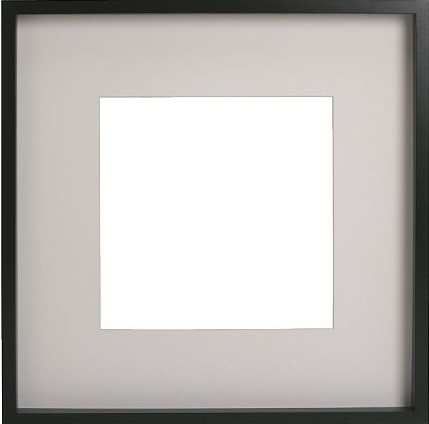
\includegraphics[scale=0.5]{bilder/ribba-rahmen-schwarz.jpg}
%	\end{center}
%	\caption{RIBBA Rahmen, schwarz}
%	\vspace{-10pt}
%\end{wrapfigure}
Die Wahl des Spiegelrahmens bedarf eines Auswahlverfahrens, da die Auswahl die weitere Vorgehensweise des Projekts bestimmt. Zur Entscheidung stehen die drei folgenden Optionen zur Verfügung. Die Basis bildet der Eigenbau, bei dem der Rahmen selbst nach seinen Bedürfnissen produziert wird. Was jedoch ein wenig handwerkliches Geschick voraussetzt. Eine weitere Möglichkeit besteht darin, den Rahmen von professioneller Seite aus, z.B. von einem lokalen Schreiner, anfertigen zu lassen. Die letzte Option beruht auf Optimierung eines bereits auf dem Markt vorhanden Produkts. Die Auswahl des Rahmens ist eng mit der Auswahl des Spiegels verflochten. Das eine entscheidet das andere. Ist der Spiegel bereits erworben, bestimmt dieser die Größe des Rahmens und verwehrt somit die Möglichkeit auf Fremdprodukte zurück zu greifen. Daher empfiehlt es sich zuerst die Anschaffung des Rahmens zu organisieren, um anschließend anhand der Rahmengröße den passenden Spiegel zu besorgen.  
\begin{table}
	\begin{tabular}{rc|cc}
		& \multicolumn{3}{r}{\textbf{Projektbudget beschränkt?}} \\
		& & ja & nein \\
		\hline
		\multirow{2}{*}{\textbf{Projektzeit beschränkt?}} & ja  & 3 & 3 \\
		& nein & 1 & 2,3 \\
	\end{tabular}
	\caption{Hilfstabelle für die Entscheidung der drei Optionen}
	$ 
	^{\textrm{1 = Eigenproduktion, 2 = Fremdproduktion, 3 = Optimierung eines Fremdprodukts}}
	$
\end{table}
Die Herstellung durch ein Subunternehmen hängt fundamental von dem Projektbudget ab. Zusätzlich wird die Option von dem Zeitfaktor entschieden. Ist das Projekt schnell zu realisieren, ist zunächst mit dem Subunternehmen zu klären, ob eine Deadline eingehalten werden kann. Sind das Projektbudget und der Zeitfaktor stark eingeschränkt, ist die Wahl der dritten Option die optimale Lösung. Als Hilfestellung dient die Tabelle 2.

Dieses Projekt beruht auf dem Einsatz eines Fremdprodukts in Abbildung 1. Der Bilderrahmen der Firma IKEA entspricht den Bedürfnissen und Anforderungen und lässt sich durch wenig Aufwand optimieren. \\
Die Größe des Rahmens ist 50 x 50 x 4,5 cm. Bedauerlicherweise stehen auf Grund der Rückwand effektiv nur 4cm der Höhe zur Verfügung. Die Rückwand ist in den Rahmen integriert und raubt somit kostbaren Platz. Die einzige Herausforderung besteht lediglich darin, die restlichen Komponenten in der begrenzten Höhe unter zubringen, was jedoch bei der richtigen Platzierung der Komponenten sehr gut gelingt. Der Preis für den Rahmen liegt bei \EUR{12,99} und ist somit eines der günstigsten Komponenten. Ideal geeignet für ein geringes Projektbudget.

Zusammengefasst gilt. Ist das Projekt schnell zu realisieren, empfiehlt sich definitiv die Verwendung des IKEA Rahmens oder eines ähnlichen Produkts. Zu beachten ist jedoch, dass die Wahl der Größe eingeschränkt ist. Hat man hingegen den Wunsch einen größeren Spiegel oder z.B. einen Spiegel für das Badezimmer mit Ablageflächen zu konstruieren, bleiben nur die beiden ersten Optionen übrig. Ist man Handwerklich begabt und hat man genügend Zeit, sowie Budget, kann man sicherlich den Bau des Rahmens selbstständig durchführen. Oder man lässt sich einen Rahmen nach seinen Bedürfnissen anfertigen.

\begin{figure}
	\vspace{-20pt}
	\begin{center}
		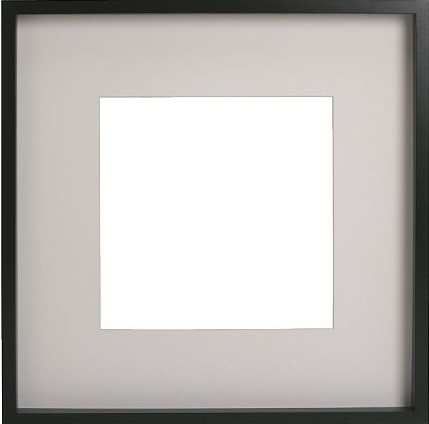
\includegraphics[scale=0.4]{bilder/ribba-rahmen-schwarz.jpg}
	\end{center}
	\caption{RIBBA Rahmen, schwarz}
	\vspace{-10pt}
\end{figure}

\subsection{Die Eigenschaften des Spionspiegels}
Die Wahl des richtigen Spiegels ist entscheidend für die Funktion des \textit{SmartMirrors}. Ebenso wie bei dem Rahmen stehen wiederum zwei Optionen zur Verfügung. Entweder wird der Spiegel mit einer professionellen Beschichtung von einem Subunternehmen erworben oder durch eine sogenannte Spionfolie in Eigenregie auf eine Glasscheibe aufgetragen. Dieser Vorgang wird auch Folieren genannt und wird im weiteren Verlauf näher beschrieben. Ein Vorteil bei der Verwendung des IKEA Rahmens ist die Glasscheibe die bereits beim Bilderrahmen mitgeliefert wird. Diese kann ohne Probleme verwendet werden und muss nicht zusätzlich angepasst werden. Das Folieren ist eine kostengünstige und schnelle Alternative, welche bei diesem Projekt eingesetzt wurde. Die Folie kostet \EUR{13,89} inkl. Versand und ist selbst mit wenig Erfahrung innerhalb von 15 min auf der Glasscheibe foliert.

\subsubsection{Die physikalischen Merkmale}
Damit der Einsatz des \textit{SmartMirrors} gelingt und das Gadget optimal genutzt werden kann, sind die Eigenschaften des Spionspiegels, auch bekannt unter dem Namen Einwegspiegel, zu erläutern. Das Besondere daran ist, das der Spiegel von einer Seite bis zu einem bestimmten Prozentsatz reflektierend ist und von der anderen Seite Lichtdurchlässig, auch unter dem Begriff Transmission bekannt. Siehe Abbildung 2. Diese Eigenschaften ermöglichen es uns auf der Rückseite des Spiegels, also im Inneren, einen Monitor anzubringen dessen Licht auf der reflektierenden Seite angezeigt wird. Dabei entscheidet das Verhältnis zwischen dem Reflexionsgrad und der Transmission über die Qualität der Anzeige. Daher empfiehlt es sich einen Spiegel mit dem Reflexionsgrad von ca. 70-80\% und einem Transmissionswert von etwa 8\% zu verwenden. 
\begin{figure}[H]
	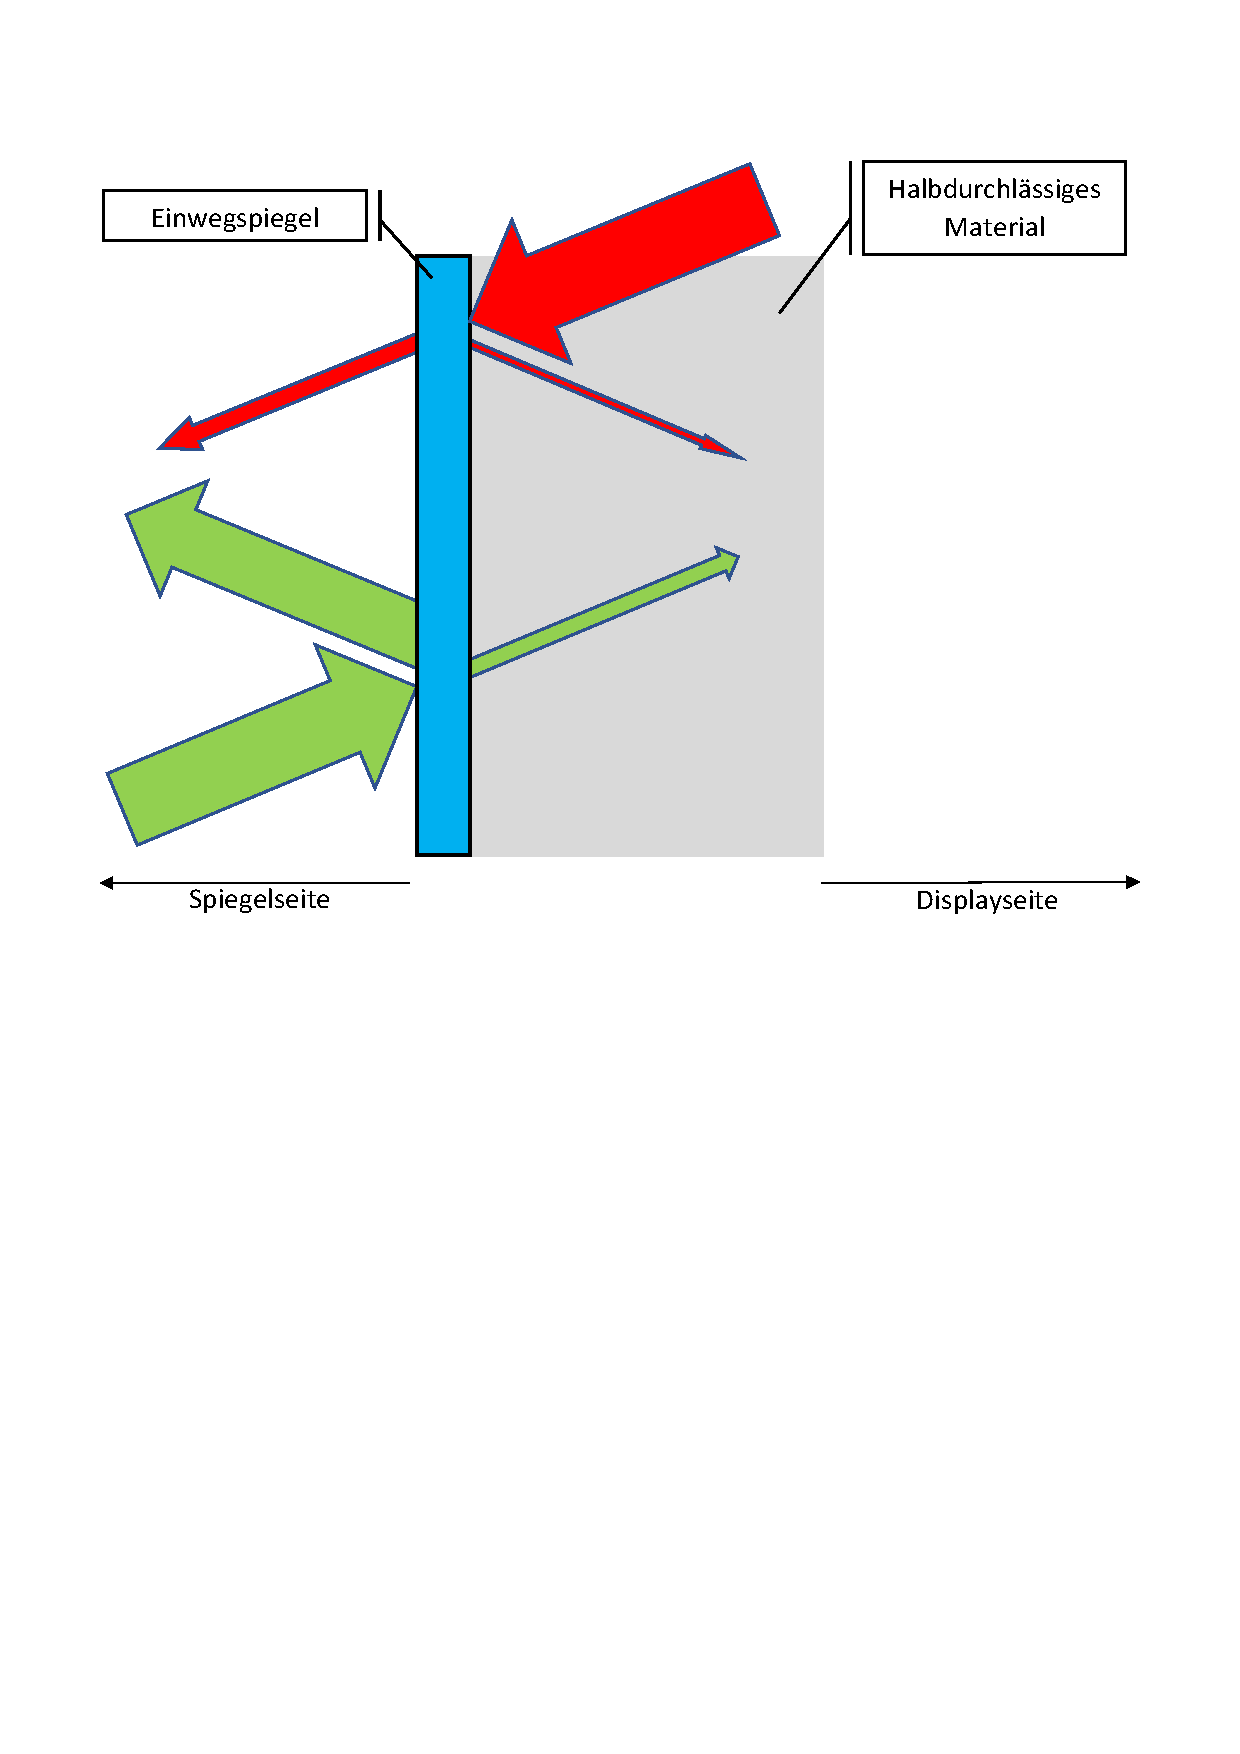
\includegraphics[trim=30mm 140mm 30mm 30mm, scale=0.45]{bilder/Einwegspiegel.pdf}\\
	\caption{Reflexions- und Transmissionswirkung}
	{\scriptsize Der rote Pfeil symbolisiert das Displaylicht und der grüne Pfeil das Umgebungslicht des Spiegels. Das Umgebungslicht wird zum größten Teil wieder reflektiert und das Displaylicht wird nahezu nach außen geleitet. }
\end{figure}

\subsubsection{Anleitung zum folieren einer Folie auf eine Glasscheibe}
Das folgende Werkzeug wird für die Folierung benötigt
\begin{center}
	\begin{singlespace}
		\begin{itemize}
			\item ein Folienrakel
			\item eine Sprühflasche mit einer Wasser-Spülmittellösung
			\item ein Cuttermesser
			\item ein Scheibentuch bzw. Microfasertuch, was am besten keine Fuseln hinterlässt.
		\end{itemize}
	\end{singlespace}
\end{center}
Steht kein Folienrakel zur Verfügung, kann das Werkzeug unter dem folgenden \href{https://www.amazon.de/Folienrakel-Filzkante-Filzrakel-Kunststoffrakel-Verkleberakel/dp/B073S7KT25/ref=sr_1_2?ie=UTF8&qid=1503417838&sr=8-2&keywords=werkzeug+folierung}{Link} bei Amazon erworben werden. Als Alternative kommt eine Kreditkarte zum Einsatz. Diese wird mit einem Brillentuch umwickelt und als Ersatz für den Folienrakel genutzt. Ersatzweise kann man statt dem Spülwasser auch Scheibenreiniger verwenden.

Um die Folie auf die Scheibe aufzutragen, sollte diese zunächst gründlich gereinigt und anschließend mit einem Fensterwischer abgezogen werden, damit soviel Staub und Schmutz wie möglich abgetragen wird. Das beste Ergebnis lässt sich erzielen, wenn der Vorgang im Badezimmer durchführt wird und kurz vorher heißes Wasser aus der Dusche durchgelaufen lassen wird. Das heiße Wasser erhöht die Luftfeuchtigkeit im Raum und senkt somit den Staubgehalt in der Luft, was zu einem besseren Ergebnis führt.

Anschließend wird die Scheibe leicht mit dem Spülwasser befeuchtet, um eine Art Gleitschicht zu erzeugen. Diese Gleitschicht erleichtert das spätere Positionieren der Folie und minimiert die Bläschenbildung. Die Folie wird ,,schwimmend`` aufgetragen.

Zunächst ist die Schutzschicht der Folie zu entfernen, sofern diese vorhanden ist. Um die Schutzschicht leichter von der Spionfolie zu lösen, werden zwei Streifen Tesafilm von beiden Seiten auf eine Ecke geklebt. Beim auseinanderziehen lösen sich die beiden Folien von einander. Dabei ist zu beachten, dass man anschließend die richtige Seite zur weiteren Bearbeitung verwendet und diese nicht beim abziehen beschädigt.

Je nach Erfahrungsgrad empfiehlt es sich definitiv etwas mehr Folie zu bestellen. Sollte beim Folieren etwas schief gehen, kann die Folie einfach wieder abgezogen und ein zweiter Versuch gestartet werden. Die Folie sollte idealerweise einige Zentimeter breiter und länger sein, als die Glasscheibe selbst. Da man die Folie zunächst positionieren muss, ist nicht zu vermeiden das Fingerabdrücke auf der Folie zusehen sind. Um diese zu entfernen, lässt man die Folie etwas überstehen und schneidet im Anschluss die Seiten mit einem Cuttermesser ab.

Optional wird für den nächsten Schritt eine zweite Person als Unterstützung benötigt. Das erleichtert den Vorgang enorm. Nachdem die Folie von der Schutzschicht getrennt wurde, wird diese auf einer Seite der Glasscheibe aufgelegt und die Luftbläschen werden mit Hilfe des Folienrakels von einer Seite zur anderen und von Innen nach Außen heraus gerakelt. Siehe Abbildung 3. Die Hilfsperson hält dabei die andere Seite der Folie etwas höher und straft diese nach Bedarf. Anschließend werden die überstehenden Seiten vorsichtig und gleichmäßig ab geschnitten  und die Luftbläschen erneut heraus gerakelt. Ist das Ergebnis zufriedenstellend, sollte die Scheibe einen Tag liegen gelassen werden, bevor diese gereinigt werden kann. Erfahrungsgemäß verflüchtigt sich das übrige Wasser unter der Folie nach einigen Tagen. Die restlichen Luftbläschen werden zum größten Teil verschwunden sein.
\begin{figure}
	\begin{center}
		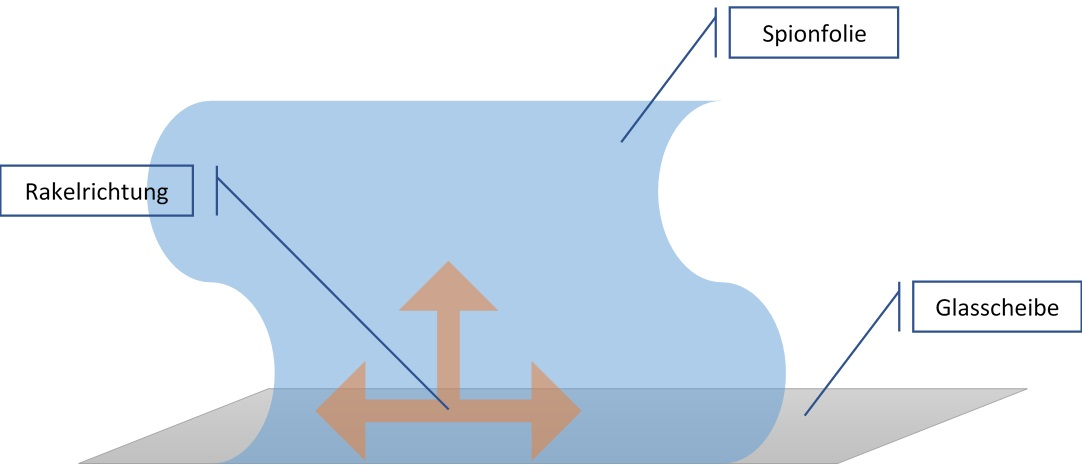
\includegraphics[scale=0.5]{bilder/Rakelanleitung.jpg}
	\end{center}
	\caption{Rakelrichtung}
	\vspace{-10pt}
\end{figure} 
\begin{figure}
	\begin{center}
		\includegraphics[scale=0.07]{bilder/spionspiegel.jpg}
	\end{center}
	\caption{Arbeitsbild der Folierung während des Proseminars}
	\vspace{-10pt}
\end{figure}

Zusammengefasst gilt, dass die Verwendung einer Spionspiegelfolie eher eine mäßig bis geradeso akzeptable Qualität bietet. Um bessere Ergebnisse zu erzielen, sollte auf eine professionell beschichtete Glasscheibe zurückgegriffen werden. Die Firma Glas Star aus Bochum hat sich auf die Herstellung der Glasscheiben für Smart Mirrors spezialisiert und bietet zahlreiche Auswahlmöglichkeiten. Die Webseite erreicht man unter dem folgenden \href{https://www.glas-star.de/spionspiegelnachmass/chrome-spy-spiegel/}{Link}. Der einzige Vorteil der Spionspiegelfolie ist der zeitliche Aspekt und die vergleichsweise niedrigen Kosten.

\subsection{Die Eigenschaften und der Einbau der Komponenten}
\subsubsection{Raspberry Pi 3}
Als Steuereinheit und Herzstück des \textit{SmartMirrors} dient ein Raspberry Pi 3 Model B. Aufgrund des integrierten WLAN-Moduls eignet sich der Raspberry Pi 3 ideal für dieses Projekt. Der \textit{SmartMirror} kann somit mobil eingesetzt werden und ist nicht fest an einen Ort gebunden. 
Für das Projekt werden lediglich einige der 40 GPIO-Anschlüsse des Boards benötigt. Es wird ein Temperatur- und Bewegungsmeldersensor angeschlossen und verwendet. Die genau Belegung der GPIO-Anschlüsse ist in Abbildung 5 grafisch dargestellt.
\begin{figure}[H]
	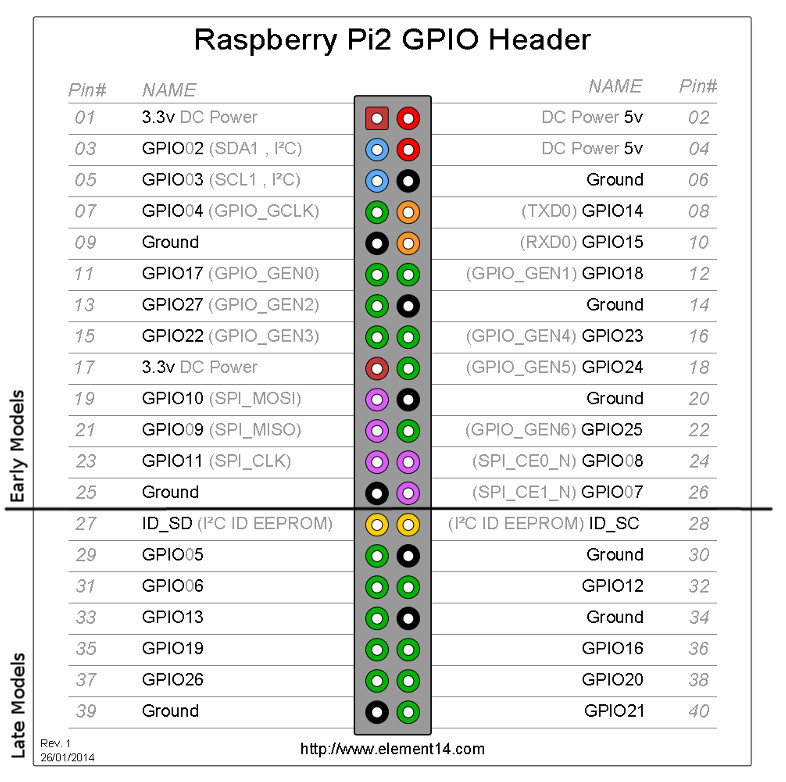
\includegraphics[scale=0.4]{bilder/gpio_pinout.jpg}
	\caption{GPIO-Belegung}
\end{figure}
Unter dem Link \url{https://www.raspberrypi.org/documentation/} ist eine ausführliche Dokumentation zu den Eigenschaften des Raspberry Pi zu finden. Da der Raspberry Pi üblicherweise ohne ein Betriebssystem geliefert wird, wird unter der bereits genannten Adresse ebenfalls eine detaillierte Installationsanleitung bereit gestellt. Für das Projekt wird als Operating System die ,,RASPBIAN JESSIE WITH DESKTOP`` Distribution verwendet. Alternativ zur Desktop Version gibt es eine Light Version. Diese ist wegen der fehlenden grafischen Oberfläche für dieses Projekt ungeeignet.

\subsubsection{Bewegungsmelder}
Als Bewegungssensor wird das Modell HC-SR501 verwendet. Der PIR-Sensor, oder auch ,,IR-Bewegungssensor`` genannt, arbeitet passiv auf Basis der Infrarotstrahlung der Umgebung.  Jeder Körper sendet eine kleine Menge an Infrarotstrahlung aus. Der PIR-Sensor stellt die Temperaturänderung im Raum fest und kann somit als Schalter verwendet werden. Der Sensor befindet sich auf einer kleinen Platine und besitzt eine einstellbare Empfindlichkeit und zwei M2 Befestigungsbohrungen für die Montage. Die Reichweite der Erfassung beträgt bis zu 7 Meter. Der Erfassungswinkel des Objektives beträgt etwa 100 Grad. 

Der Sensor ermöglicht es je nach Bedarf das Display anzusteuern und somit Energie zu sparen. Betritt eine Person den Raum, indem der Spiegel hängt, gibt der Sensor ein Signal zum Einschalten des Displays. Andernfalls bleibt das Display ausgeschaltet. 

Zum anschließen des Sensors an den Raspberry Pi 3 werden zusätzlich drei Jumperkabel benötigt. Alternativ dazu kann ein dreiadriges Kabel verwendet werden. Die Anschlüsse werden wie folgt verbunden und sind auf dem Sensor beschriftet. 
\begin{center}
	\begin{singlespace}
		\begin{itemize}
			\item VCC an Pin 2 (5V)
			\item OUT an Pin 16 (GPIO 23)
			\item GND an Pin 6 (Ground)
		\end{itemize}
	\end{singlespace}
\end{center} 
\begin{figure}[H]
	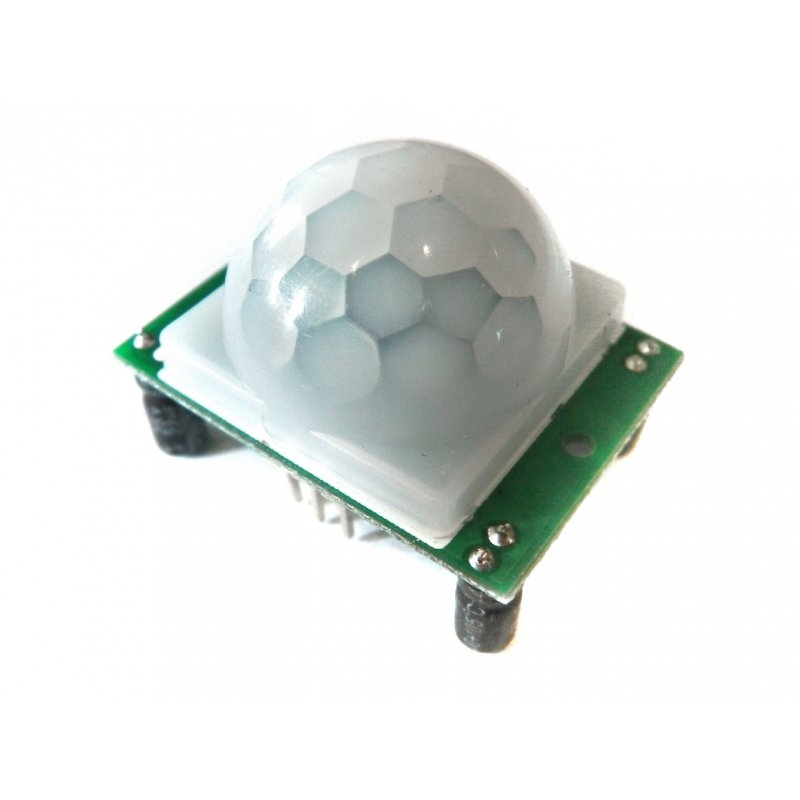
\includegraphics[trim=20mm 20mm 20mm 20mm, scale=0.2]{bilder/PIR-Sensor.jpg}
	\caption{PIR-Sensor HC-SR501}
\end{figure}

\subsubsection{Temperatur- und Luftfeuchtigkeitssensor}
\begin{figure}[H]
	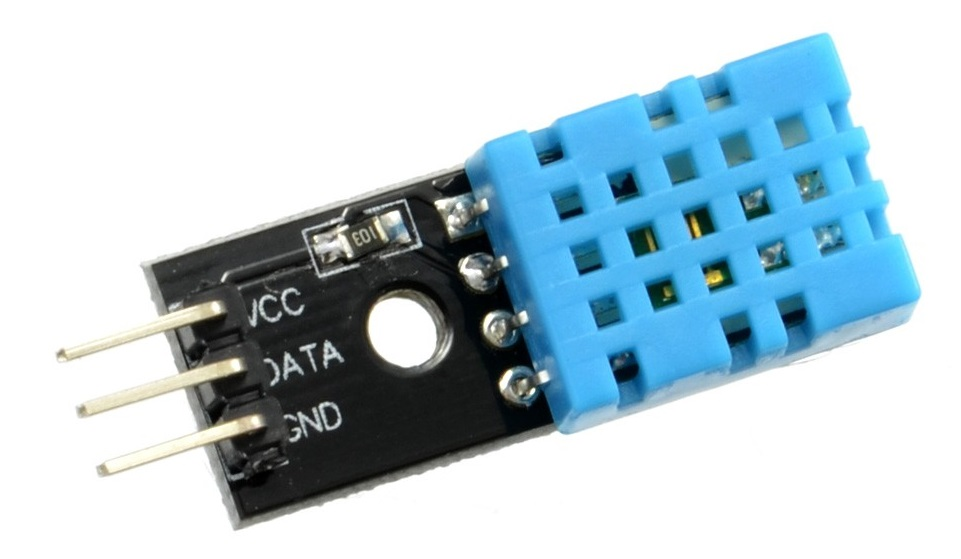
\includegraphics[trim=0mm 0mm 0mm 0mm, scale=0.3]{bilder/DHT11.jpg}
	\caption{TL-Sensor DHT11}
\end{figure}
Mit dem Raspberry Pi und dem Sensor DHT11 ist es mit wenig Aufwand möglich, sich die aktuelle Raumtemperatur und Luftfeuchtigkeit ausgeben zulassen. Da der Sensor bereits alles zur Verwendung liefert, muss dieser nur an das Board passend angeschlossen werden. Der linke Pin (VCC) des Sensors wird an den Pin1 (3.3V) des Pi´s angeschlossen. Der mittlere Sensor Pin (DATA)  ermöglicht den Datenaustausch und wird mit einen freien GPIO Pin des Raspberry Pi´s (z.B. Pin7) verbunden. Der rechte Sensor Pin (GND) muss mit einem der Ground Pin´s (z.B. Pin5) des Raspberry Pi´s verbunden werden. Die Abbildung 8 illustriert den Anschluss des Sensors an ein Raspberry Pi bei Verwendung einer Steckplatine. Anzumerken ist, dass der linke und mittlere Anschluss in der Abbildung vertauscht sind.
\begin{figure}[H]
	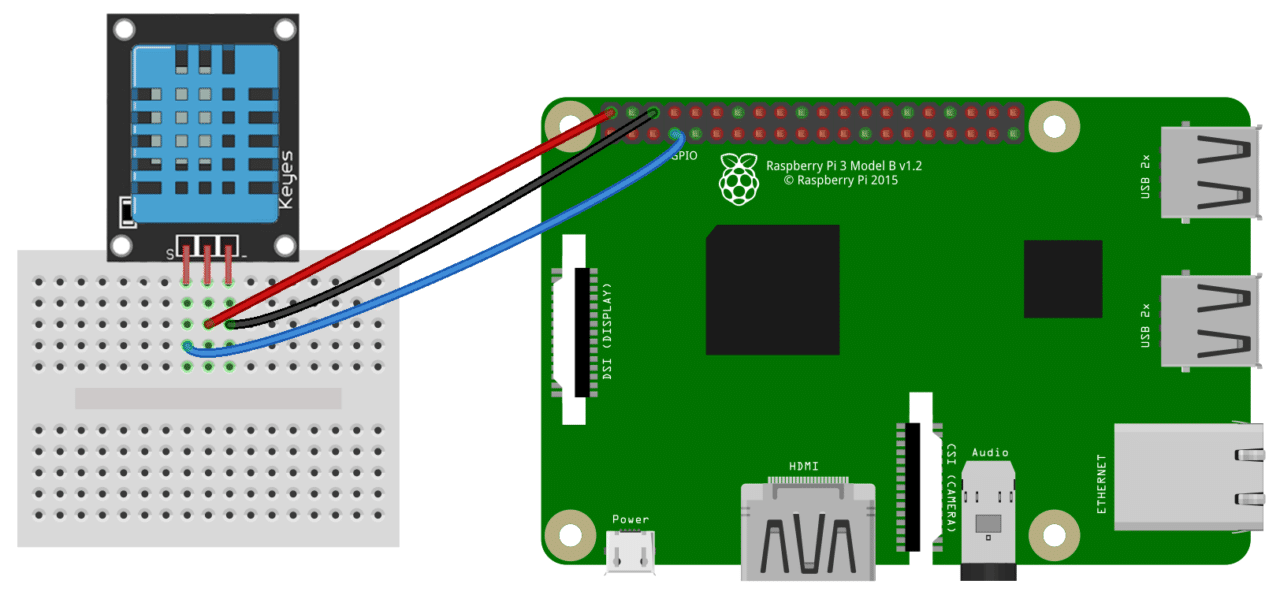
\includegraphics[trim=0mm 0mm 0mm 0mm, scale=1]{bilder/DHT11-on-the-Raspberry-Pi.png}
	\caption{DHT11 angeschlossen an ein Raspberry Pi}
\end{figure}

\subsubsection{Display}
Um dem Benutzer alle gesammelten Daten anzeigen zulassen, wird ein Display benötigt. Bei der Wahl des Displays sind einige Faktoren entscheidend. Wie bereits in Kapitel 2.1 erwähnt, steht der finanzielle Spielraum im Vordergrund. Daneben sind die Auflösung und die Stromversorgung ein wichtiger Aspekt. Für das Projekt wurde ein Acer V176Lbmd Monitor mit einer Diagonale von 17' verwendet. Der Monitor ist mit einem DVI und VGA Anschluss ausgestattet. Als Auswahl stehen zwei verschiedene Optionen für die Umsetzung des Projekts zur Verfügung. Wird ein handelsüblicher Monitor verwendet, muss dieser in die Einzelteile zerlegt werden. Alternativ können diese Komponenten einzeln erworben werden. Dabei muss die Kompatibilität unter den Bauteilen beachtet werden.  Meist besteht der Monitor aus einem Display, einem Display Controller und einem Netzteil, welches für die Stromversorgung der Bauteile zuständig ist. Das Display ist von der eingesetzten Technologie abhängig, dazu zählen z.B. LCD oder OLED Displays. Um ein Optimales Ergebnis zu erzielen, wird der Einsatz eines OLED Displays empfohlen. Dieser hat den Vorteil, dass er ein enorm starken Schwarzwert besitzt. Je nach dem wie viel Platz im inneren des Rahmens vorhanden ist, fällt die Wahl des Monitors relativ klein oder groß aus. Der Display Controller wandelt das Ausgangssignal des Raspberry Pi um und leitet die Informationen über einen 40 Pin LVDS Anschluss an das Display weiter (Abbildung 9). Einige Display Controller besitzen lediglich einen VGA Anschluss. Daher wird für das Displaysignal zusätzlich ein HDMI zu VGA Adapter benötigt, da der Raspberry Pi nur über einen HDMI Anschluss verfügt. Der besagte Adapter wandelt lediglich das Signal passend um.
\begin{figure}[H]
	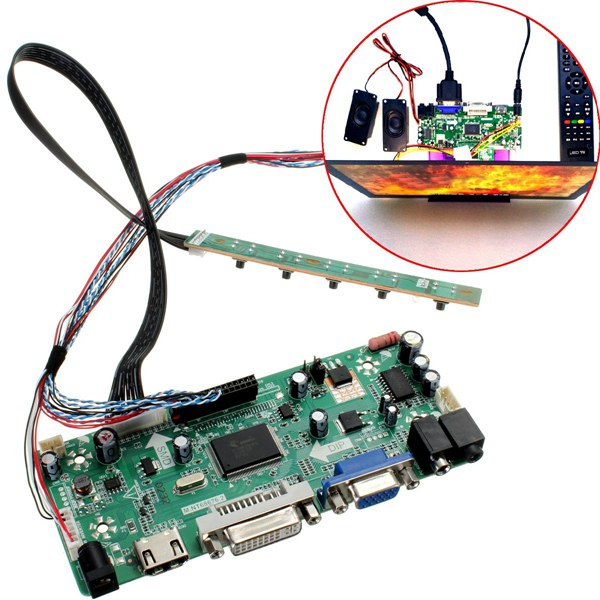
\includegraphics[trim=0mm 0mm 0mm 0mm, scale=1]{bilder/dcontroller.jpg}
	\caption{LCD Controller Board 40P}
\end{figure}

\subsection{Die praktische Umsetzung des Projekts}
Die Abbildung 10 zeigt einen Überblick über die Anordnung und Platzierung der verbauten Komponenten. Da das Display den meisten Platz veranschlagt, müssen die übrigen Komponenten um das Display herum untergebracht werden. Es wird empfohlen das Display mit einem minimalen Abstand zur oberen Kante des Rahmens zu verbauen, damit der Spiegel je nach Form nicht zu weit nach oben gehangen werden muss. Damit die Komponenten, insbesondere das Display, einen besseren halt bekommt, wurden die Komponenten mit Hilfe einer Hartschaumplatte gestützt. Dabei wurde ein Loch passend zur Größe des Displays ausgeschnitten und die anderen Komponenten auf der Platte platziert. Die Hartschaumplatte und die Rückwand sollten für ein besseres Ergebnis des Spionspiegels von innen schwarz lackiert werden (Abbildung 12-13). Die dunkle Farbe absorbiert das eintretende Licht und vermindert die Reflexion. Ein Abbild der Rückseite wird in Abbildung 11 repräsentiert.

\begin{figure}
	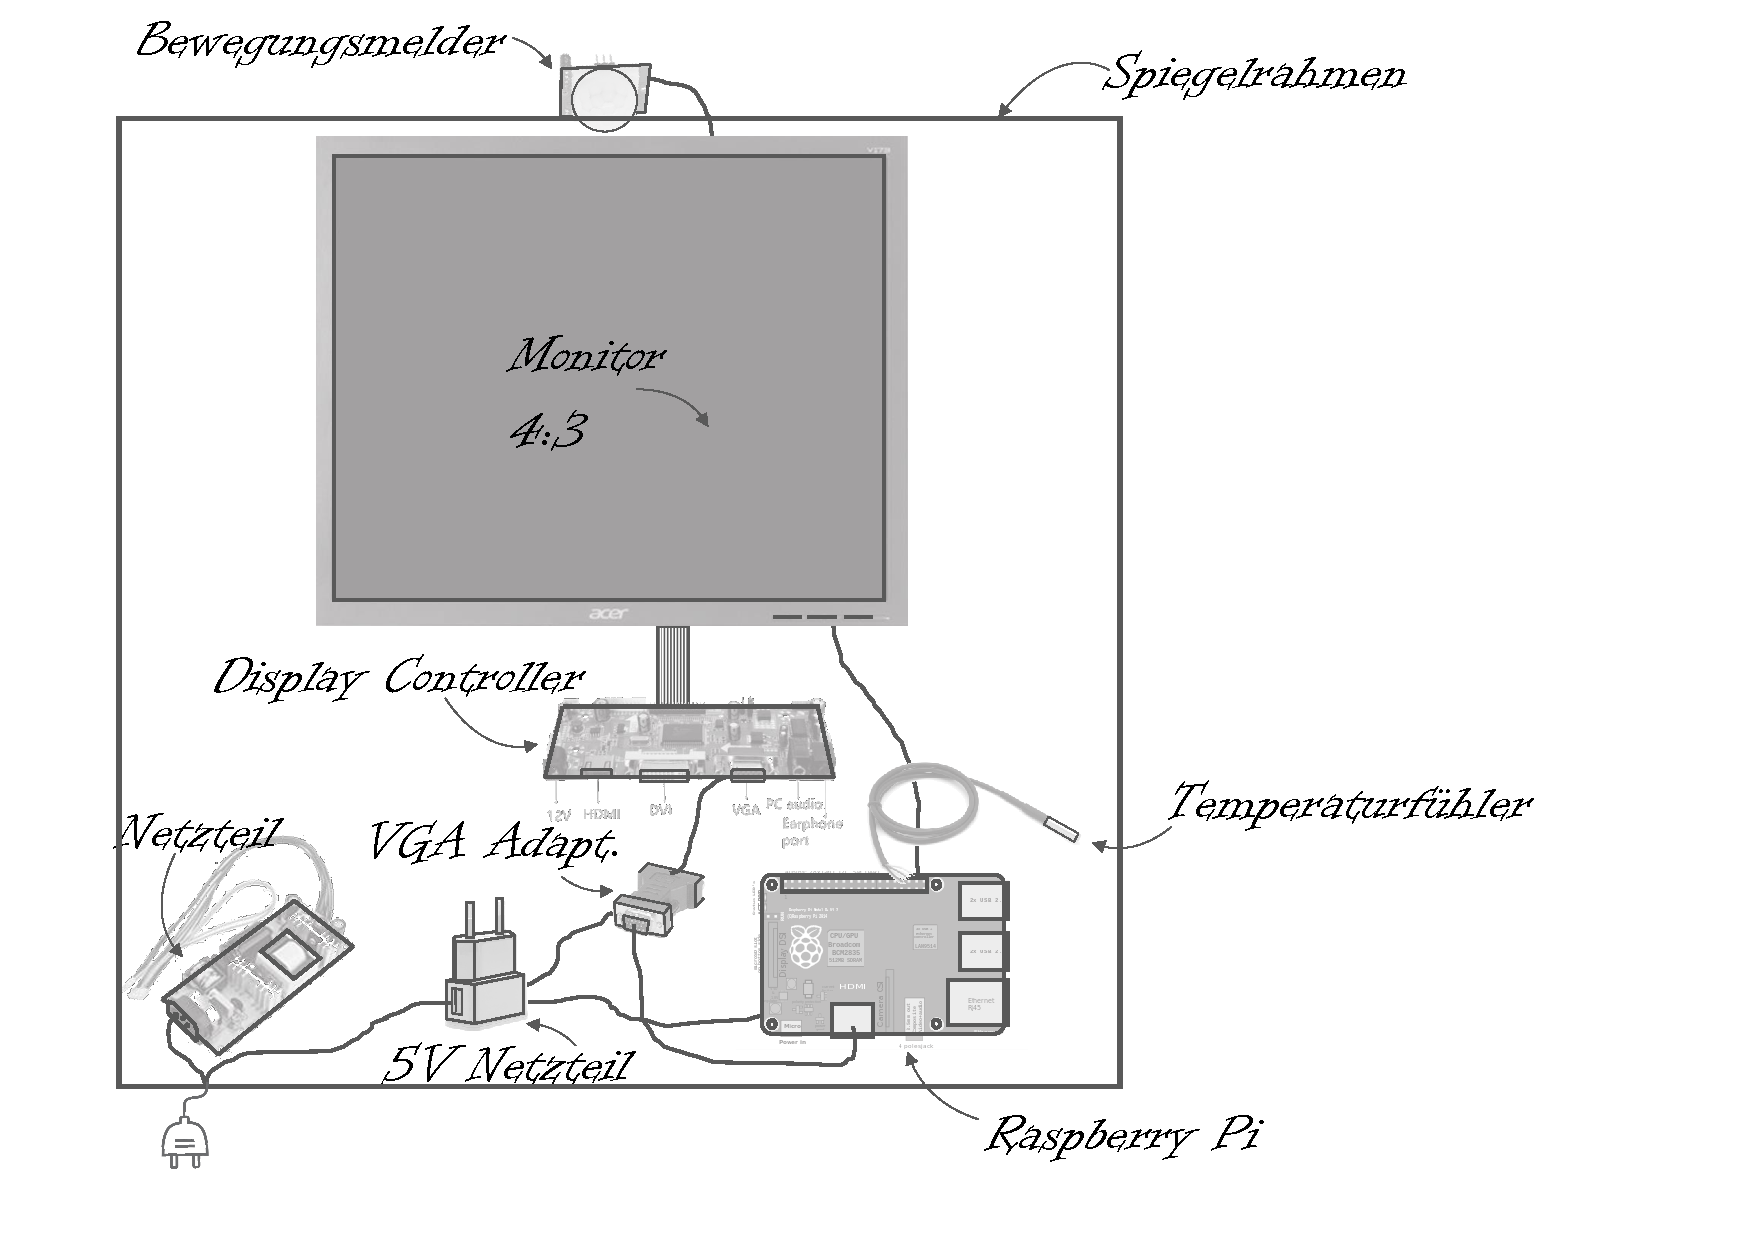
\includegraphics[scale=0.5, trim=0mm 10mm 60mm 10mm]{bilder/smartMirrorExplosionsskizze.pdf}
	\caption{Konstruktionsskizze}
\end{figure}
\begin{figure}[H]
	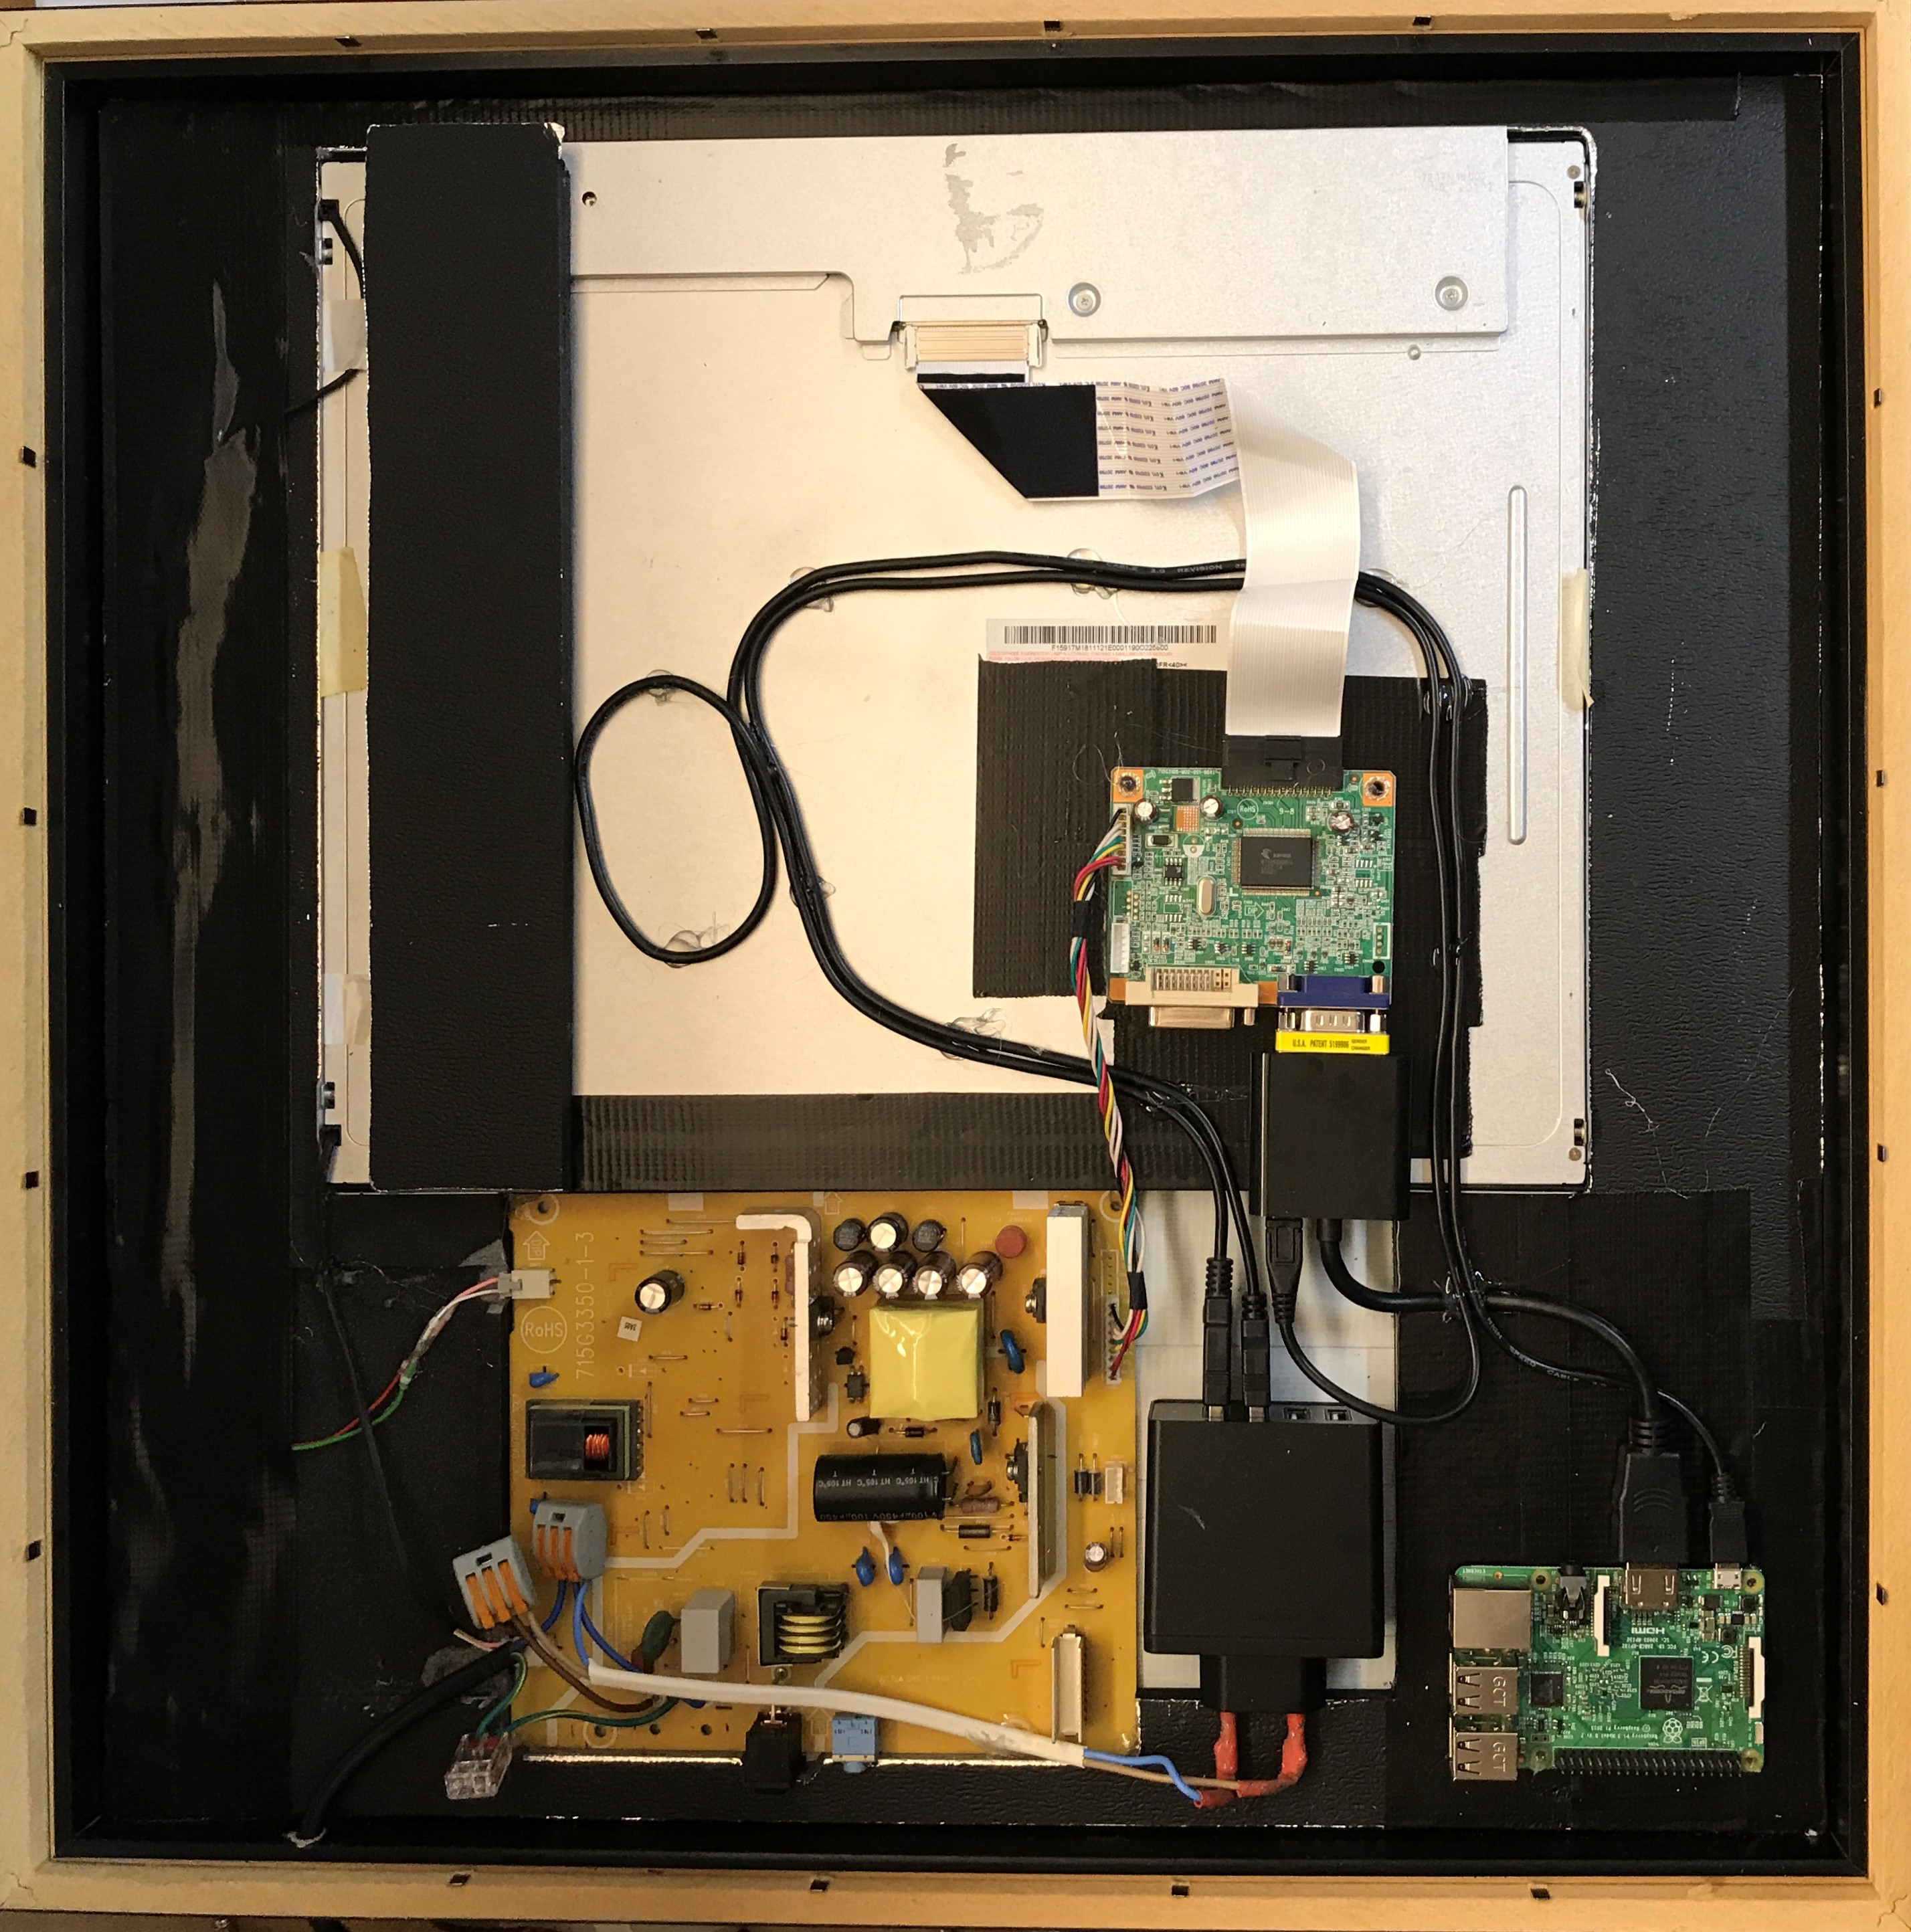
\includegraphics[scale=0.06]{bilder/Innenansicht.jpg}
	\caption{Anordnung und Verkabelung der Komponenten}
\end{figure}
\begin{figure}[H]
	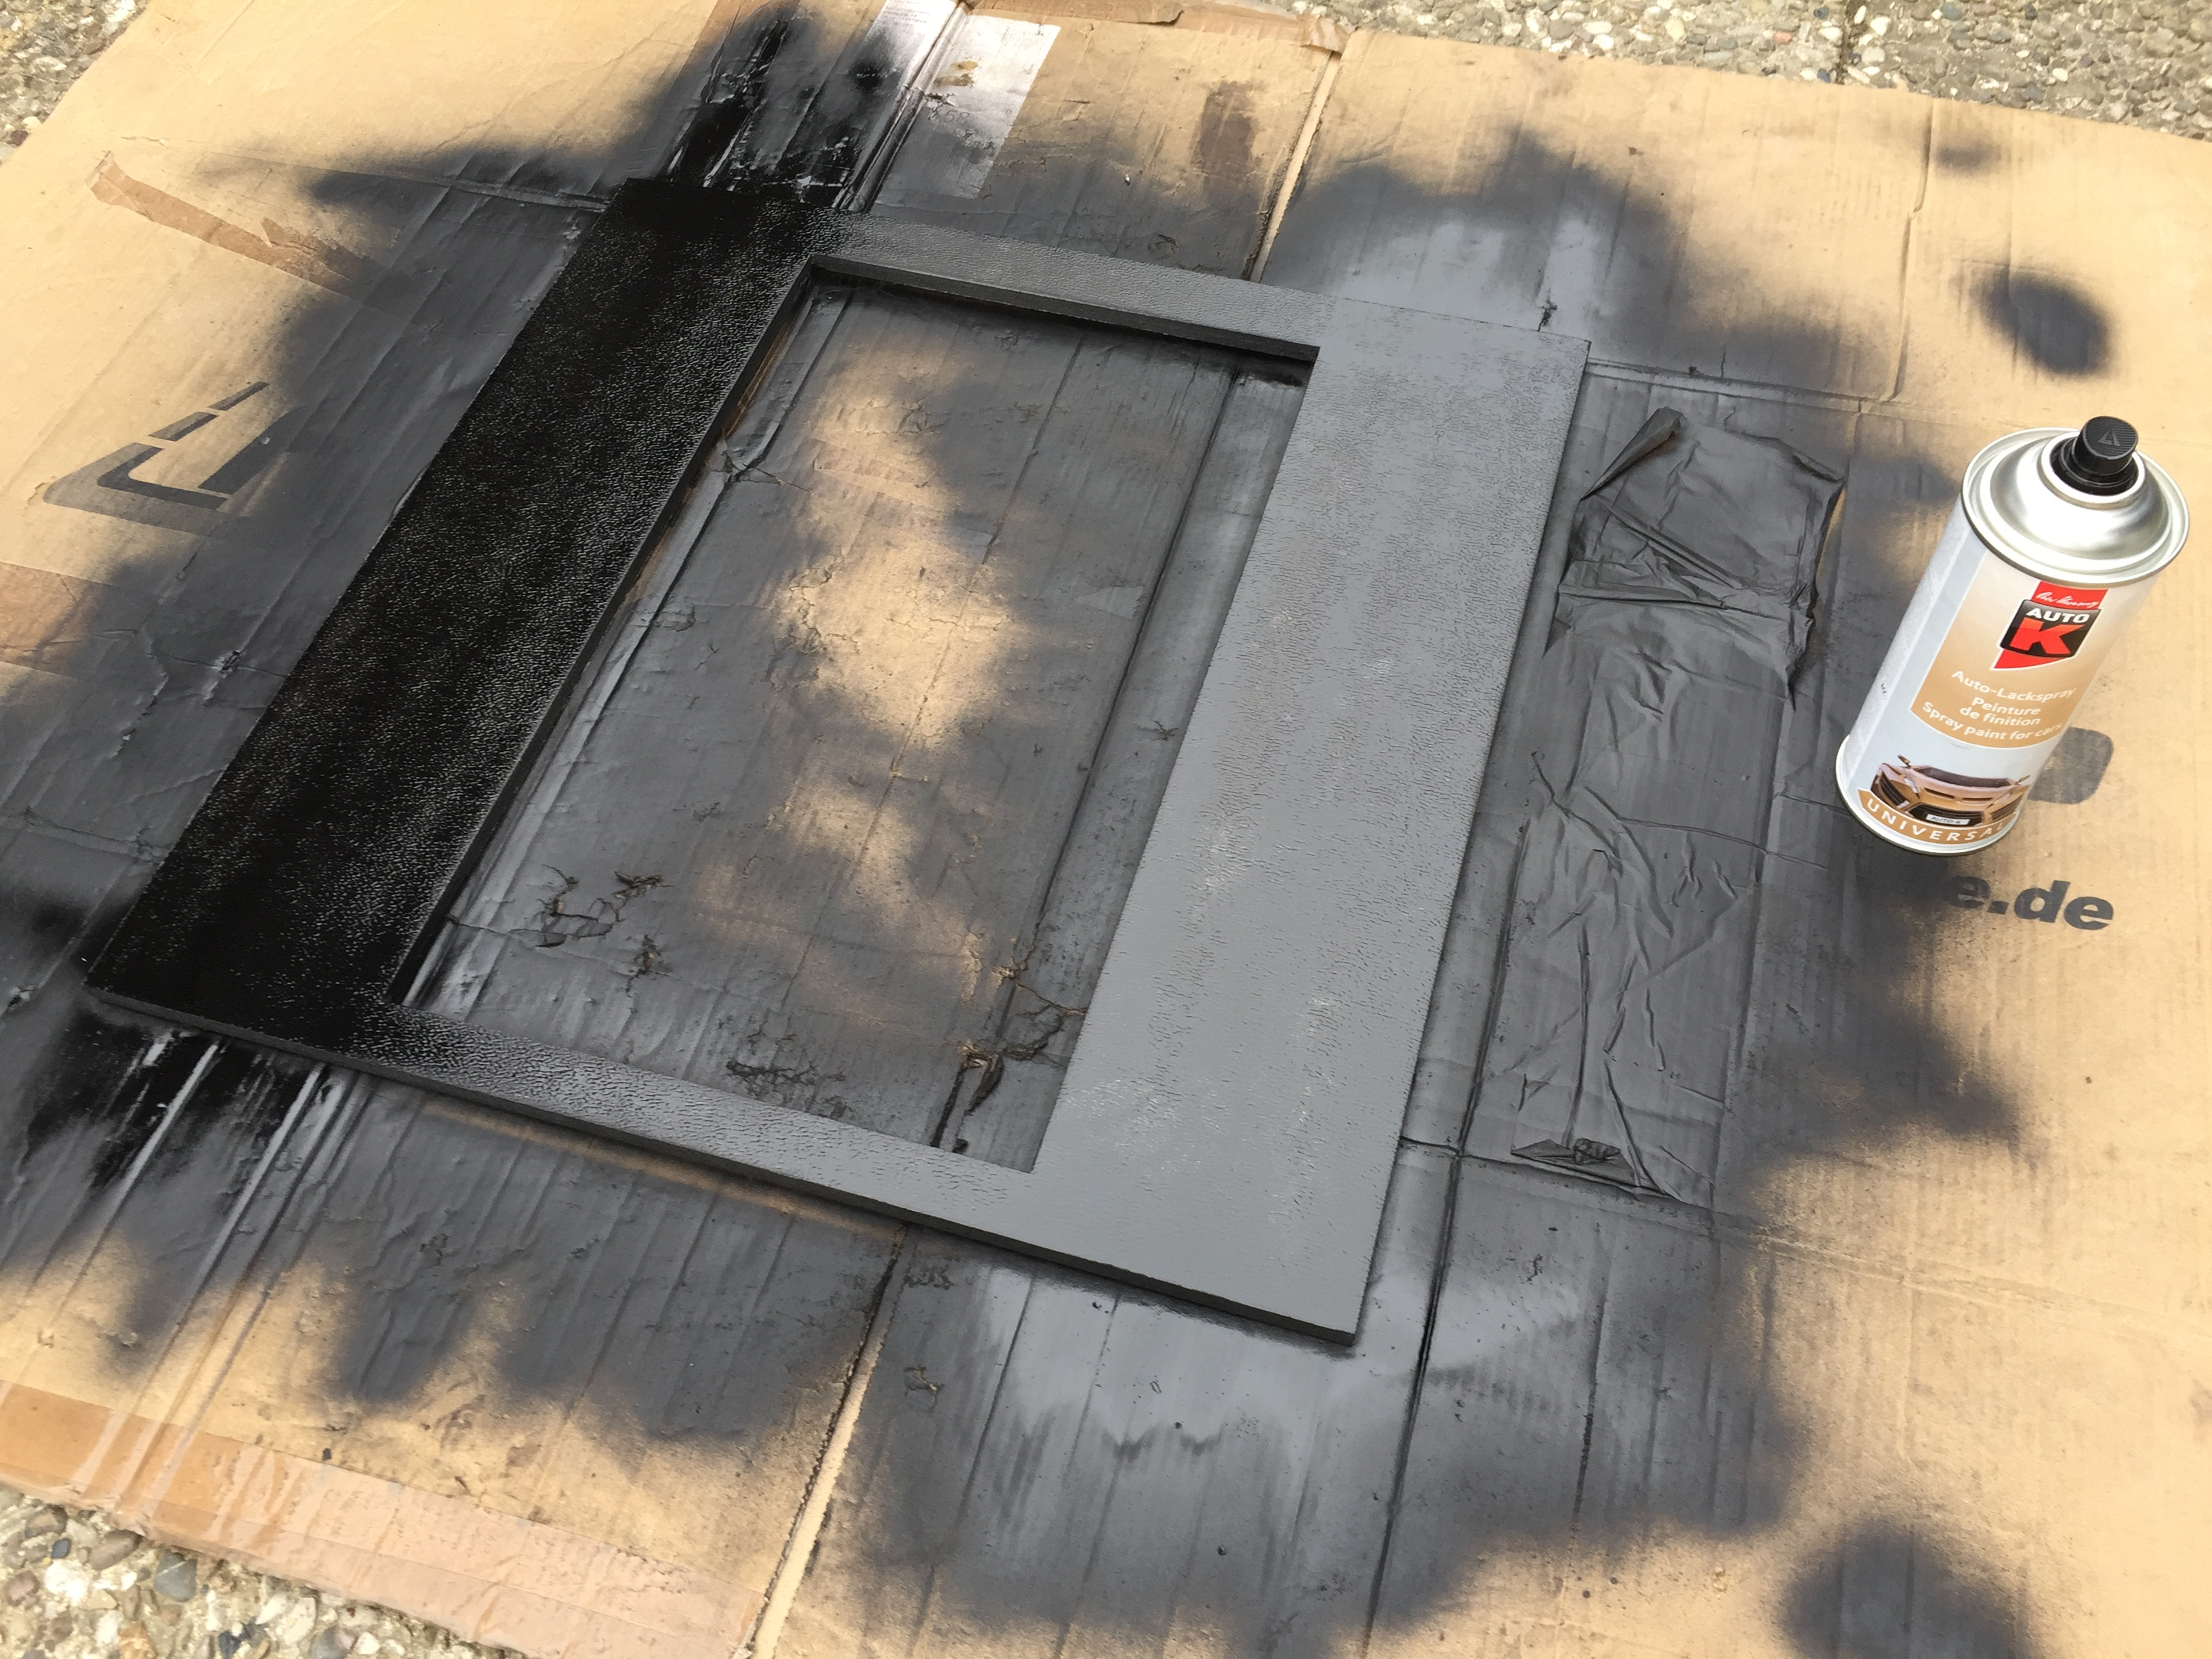
\includegraphics[scale=0.06]{bilder/Hartschaumplatte.jpg}
	\caption{Lackierung der Hartschaumplatte}
\end{figure}
\begin{figure}[H]
	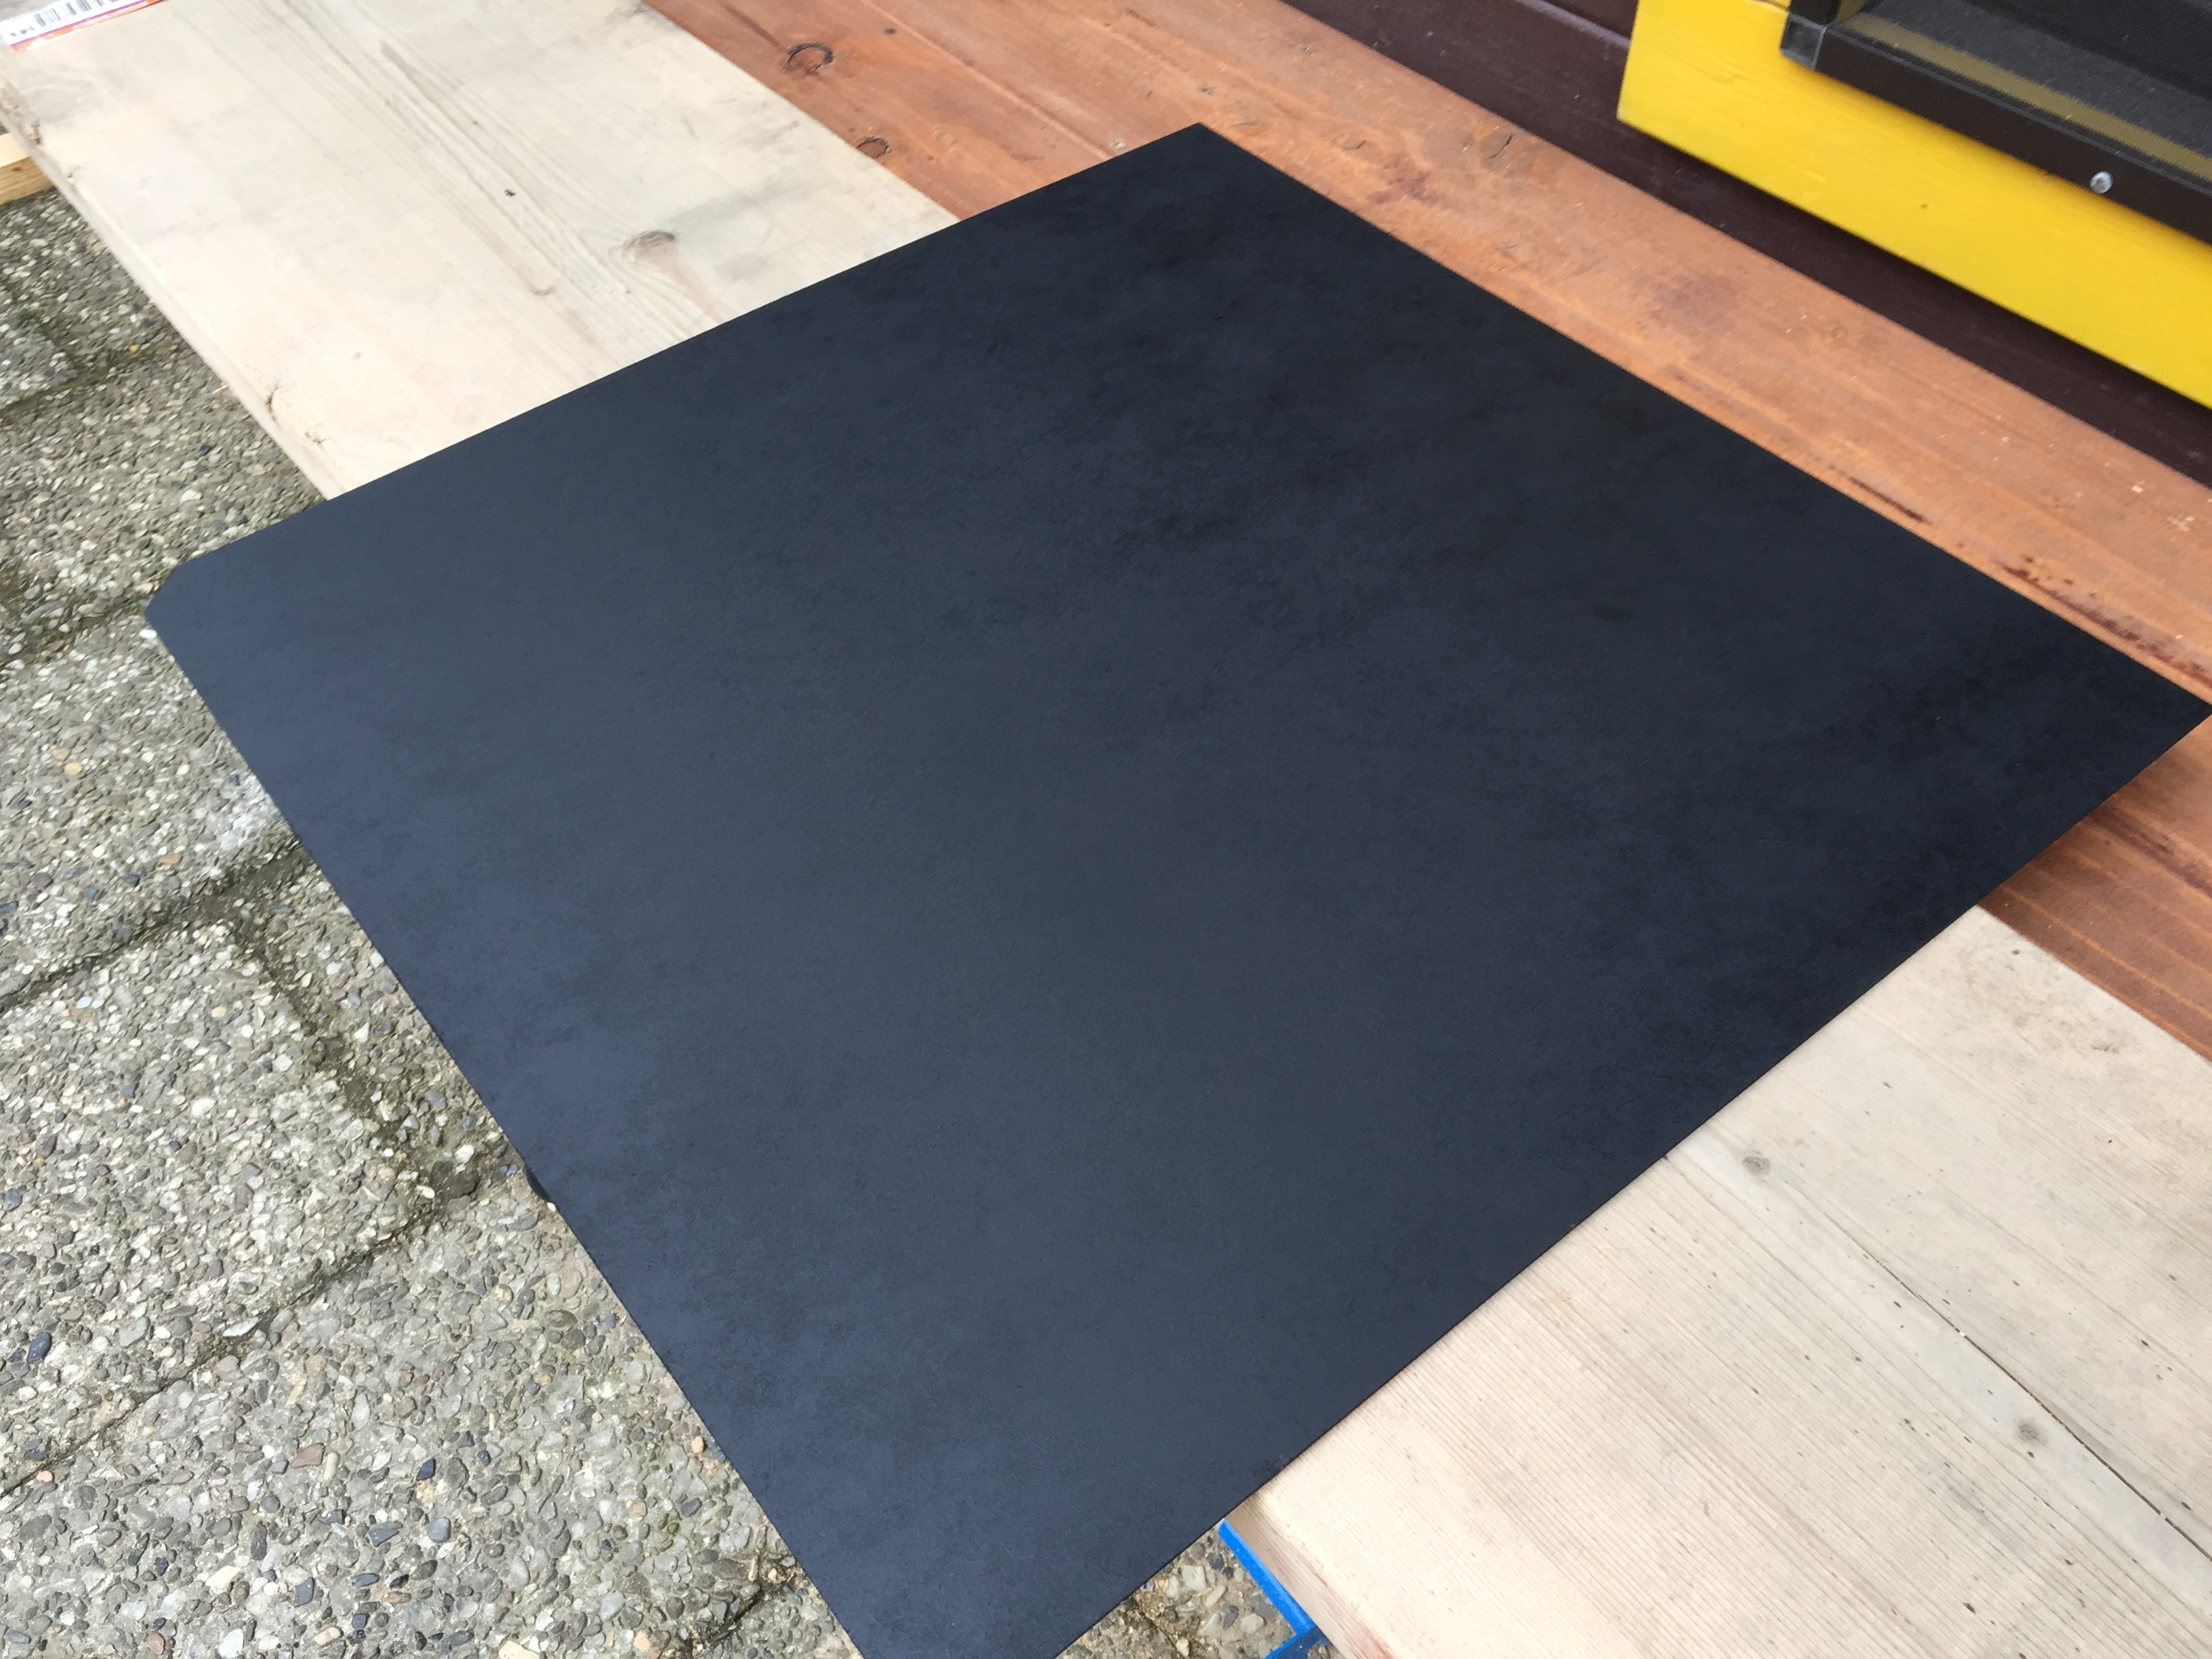
\includegraphics[scale=0.06]{bilder/Rueckwand.jpg}
	\caption{Lackierung der Rückwand}
\end{figure}
